% Section explaining the theory governing the experiment

A compound pendulum (also known as a physical pendulum) consists of a \textbf{rigid} body oscillating about a pivot. This experiment uses a uniform metallic bar with holes/slots cut down the middle at regular intervals. The bar can be hung from any one of these holes allowing us to change the location of the pivot.

\section*{Objective}

Derive an equation for the time period $T$ of the oscillations of a uniform metallic bar suspended from a pivot passing through it.

\section*{Experimental Setup}

   The experimental equipment consists of a thin uniform metallic bar with holes/slots placed through it at regular intervals. By allowing the bar to swing from different slots one can change the moment of inertia and consequently the Time Period of oscillations.

   \tikzsetnextfilename{setup}
\begin{center}
   \begin{tikzpicture}

       \def\r{5}       % Radius of the string. This definition is used in the code that we input from diag/setup-common below

       \input{diag/setup-common}

       \dimline[offset=-0.5cm, delta=0.5cm]{(bc)}{(0,0)}{$l$};

   \end{tikzpicture}
\end{center}
        % Include tex code for the diagram of the experimental setup

   We define the total length of the bar as $L$ and the distance from the pivot to the center of mass (CM) of the bar to be $l$ as indicated in the diagram above. The position of the bar at any instant of time is given by the angle $\theta$. When allowed to swing the bar performs an approximation of simple harmonic motion, that is, the angle $\theta$ varies in a cyclic fashion with time period $T$.

\section*{Free-Body Diagram}

   To calculate the time period $T$ one has to derive the equation of motion $\theta(t)$, namely how the angle $\theta$ varies as a function of time $t$. The first step, as always, is drawing the extended free body diagram of the system (extended because we are dealing with a rotational system and therefore the distance from the pivot is significant).

   \begin{tikzpicture}

   %\helpgrid{-4}{-6}{3}{2}      % Draw a grid to help place objects. Comment out in final version.
   
   \def\b{-5.5}         % Variable containing the position of the bottom of the bar
   \def\hw{0.2cm}       % Half-width of the bar
   \def\r{0.05}         % Radius of the pin-hole circles in the bar
   \def\cy{-2.25}       % Vertical position of center of bar

   \draw [dashed] (0,1) -- (0, \b);       % Dashed vertical line representing the equilibrium position. Note use of the variable \b

   \draw [rotate around={-30:(0,0)}]      % Rotate the following constructed object (bar with holes) about the origin by -30 degrees

      (0,1) -- (0,\b)       % The thick line representing the bar

      [thick, fill]                     % These attributes will be applied to the circles that follow
      (0,0) circle [radius=\r]          % Draw a thick point to represent the pivot
      (0,\cy) circle [radius=\r]        % Draw a thick point to represent the Center of Mass
   ;

   % Show angle theta using an arc with an arrow
   \def\ar{1}         % Radius of arc used to define angle
   \draw [->,>=stealth] (0, -\ar) arc (-90:-120:\ar);           % Draw an arc with an arrow at the end for the angle
   \draw (-100:\ar+0.25) node {$\theta$};                       % Note the use of polar coordinates to place the variable theta

   \dimline[offset = -0.5cm, show extensions = false]{(-120:-\cy)}{(0,0)}{$l$};

\end{tikzpicture}


   There are two forces acting on the bar. Its weight, which acts at the bar's center of mass/gravity, and a force of unknown magnitude and direction acting at the pivot, $\vec{F}_p$.
   
\section*{Derivation}
   
   We are interested in calculating $\theta(t)$ so we focus on the rotation of the bar about the \textbf{pivot} and calculate torque. Since the unknown force $\vec{F}_p$ acts at the pivot, its torque about the pivot is zero (moment-arm has zero length). Therefore only the weight $m g$ appears in our calculations. The torque is given by
   \beq \label{tau_weight}
      \tau = - m g l \sin(\theta)
   \eeq
   where the negative sign denotes the fact that the rotational direction of the torque is always opposite to that of the angle. For instance in the free-body diagram the angle $\theta$ is counter-clockwise while the torque exerted by the weight is in the clockwise direction.

   The effect of this torque is to produce angular acceleration according the Newton's Second Law of Motion:
   \beq \label{tau_alpha}
      \tau = I \alpha
   \eeq
   %
   \newcommand{\dTtheta}{\ensuremath{\frac{d^2 \theta}{dt^2}}}
   %
   where $I$ is the moment of inertia of the bar about the pivot and $\alpha = \dTtheta$ is its angular acceleration. Note that since $I$ is calculated about the pivot it is a function of the distance $l$.

   \vspace{\baselineskip} 
   Substituting equations \eqref{tau_weight} and $\alpha = \dTtheta$ into \eqref{tau_alpha}:
   %
   \beqcn
      \tau = I \alpha\\
      \imply - m g l \sin(\theta) = I \alpha\\
      \imply \alpha = - \frac{m g l}{I} \sin(\theta)\\
      \imply \dTtheta = - \frac{m g l}{I} \sin(\theta)\\
   \eeqcn

   This is a differential equation which needs to be solved for the function $\theta(t)$. In its current form it has no analytical solution. However if we limit the system to small angles $\theta \ll 1$, that is only allow small-angle oscillations (small amplitude) we can make the approximation 
   \beqn
      \theta \ll 1 \imply \sin(\theta) \approx \theta
   \eeqn
   which transforms the differential equation in to
   \beq \label{diffeqn}
      \dTtheta = - \frac{m g l}{I} \theta
   \eeq

   This differential equation has the well-known form $\frac{d^2 x}{dt^2} = - \omega^2 x$ with the equally well-known solution $x(t) = x_0 \sin(\omega t + \phi)$. $\omega = \frac{2 \pi}{T}$ is the angular frequency of the system while $T$ is its time period. The solution $x(t)$ of the differential equation is sketched below. Note its periodic behavior. The motion of the swinging compound pendulum is similar, it swings back and forth, taking the same amount of time ($T$) to complete each oscillation.
   
   \vspace{0.5\baselineskip}
      \begin{center}
      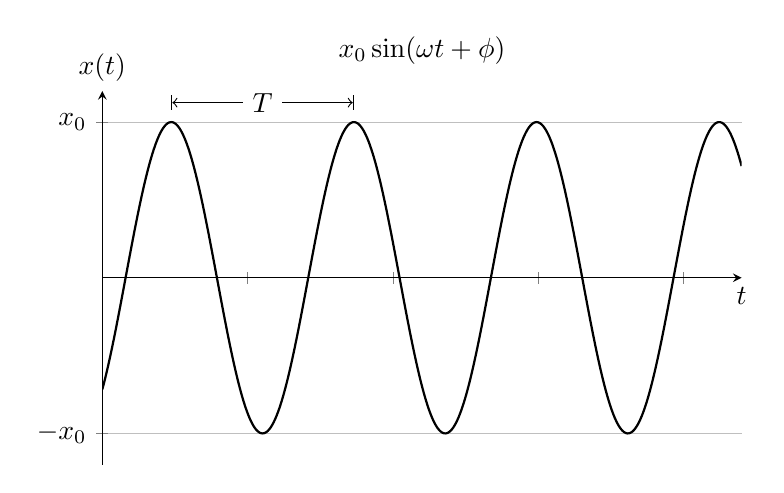
\begin{tikzpicture}

         \def\dx{0.8}

         \begin{axis}[
            width = 0.8\textwidth,
            height = 15\baselineskip,
            axis lines= middle, 
            xlabel=$t$, 
            every axis x label/.style={at={(current axis.right of origin)}, anchor=north},
            every axis y label/.style={at={(current axis.north west)}, anchor=south},
            ylabel=$x(t)$, 
            title={$x_0 \sin(\omega t + \phi)$}, 
            ymin = -1.2, 
            ymax = 1.2,
            ytick={1,-1},
            yticklabels={$x_0$, $- x_0$},
            ymajorgrids,
            xtick={},
            xticklabels={},
            ]

            
            \addplot[domain=-0:7*pi, samples=500, thick]{sin(deg(x - \dx))};
            \draw[|<->|] (axis cs: 0.5*pi + \dx, 1.125) -- node[fill=white]{$T$} (axis cs: 2.5*pi + \dx, 1.125);

         \end{axis}
      \end{tikzpicture}
   \end{center}

   \vspace{0.5\baselineskip}
   
   By simply inspecting \eqref{diffeqn} and comparing with the general form $\frac{d^2 x}{dt^2} = - \omega^2 x$ we can conclude that
   \beqc \label{T_I}
      \omega^2 = \frac{m g l}{I}\\
      \imply \big( \frac{2 \pi}{T} \big)^2 = \frac{m g l}{I}\\
      \imply T = 2 \pi \sqrt{\frac{I}{m g l}}
   \eeqc



   The final step is to calculate $I$ for a given value of $l$. For this we use the parallel axis theorem. If the mass of the bar is $m$ then $I$ is given by
   \beq \label{parallel_axis}
      I = I_{CM} + m \, l^2
   \eeq
   where $I_{CM}$ is the moment of inertia of the bar about its center of mass and $l$ is the distance from the pivot to the center of mass. In turn, $I_{CM}$ is calculated by considering the bar to have negligible width and uniform mass distribution, in which case the moment of inertia is known to be given by:
   \beq \label{ICM}
      I_{CM} = \frac{1}{12} \, m \, L^2
   \eeq
   where $L$ is the total length of the bar.

   Substituting \eqref{parallel_axis} and \eqref{ICM} in to \eqref{T_I}
   \beqc
      T = 2 \pi \sqrt{\frac{I}{m g l}}\\
      \imply T = 2 \pi \sqrt{\frac{I_{CM} + m \, l^2}{m g l}}\\
      \imply T = 2 \pi \sqrt{\frac{\frac{1}{12} \, m \, L^2 + m \, l^2}{m g l}}\\
      \imply T = 2 \pi \sqrt{\frac{L^2 + 12 l^2}{12 g l}}
   \eeqc

   Thus we achieve our objective by deriving an equation that relates the time period $T$ of a compound pendulum to its physical characteristics, mainly its total length $L$ and the distance $l$ from the pivot to the bar's center of mass, and to the acceleration of gravity.
